\chapter{User Manual}

\begin{figure}[H]
	\centering
	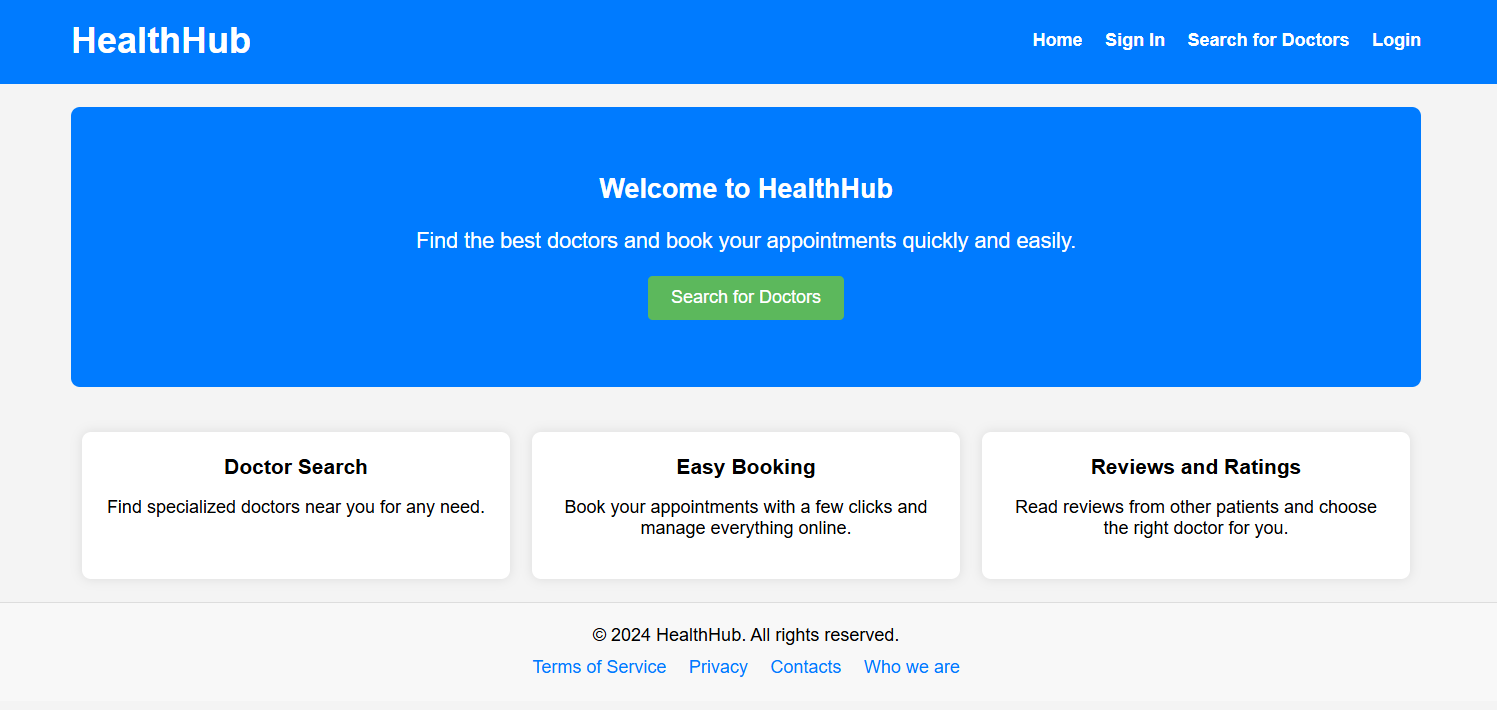
\includegraphics[width=0.8\textwidth]{resources/screenshots/homepage.png}
	\caption{Home Page of the HealthHub Application}
	\label{fig:homepage}
\end{figure}

\section{Patient}
From the Home Page you can go to the "\textit{Sign In}" option in the top right of the page. 


\section{Doctor}

Doctors have access to a dedicated interface that allows them to manage their appointments, review patient feedback, and edit their personal and professional information. They can also monitor key analytics related to their activity and configure their weekly availability through calendar templates.

\subsection{Dashboard}

\begin{figure}[!h]
    \centering
	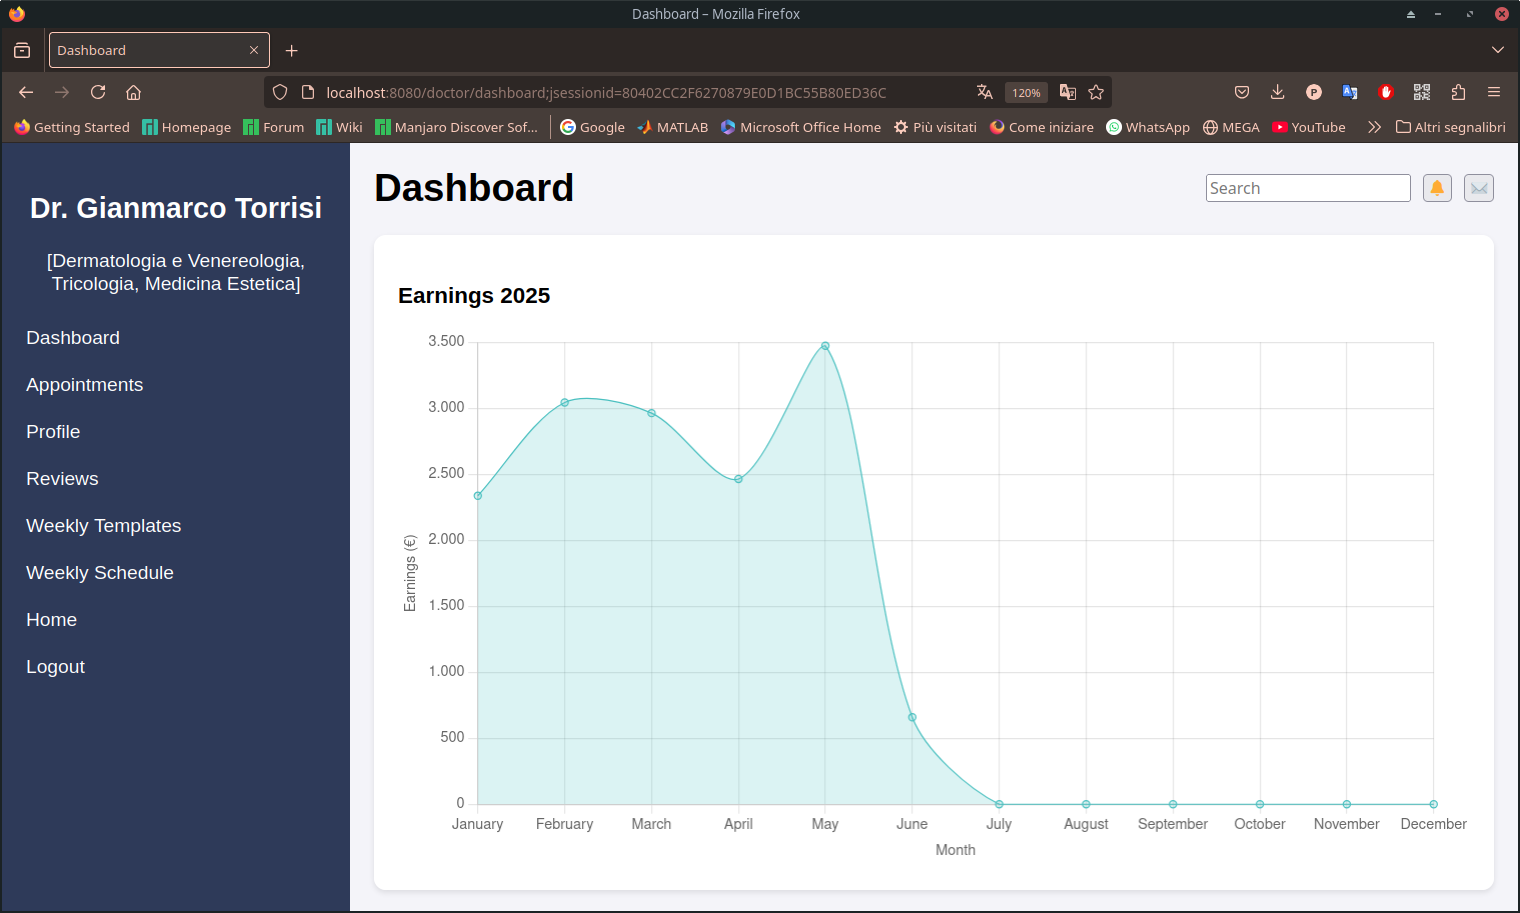
\includegraphics[scale=0.30]{resources/screenshots/doctor_ui/earnings_linechart.png}
    \caption{Line chart displaying earnings by month for the current year.}
    \label{fig:earnings_linechart}
\end{figure}

\begin{figure}[!h]
    \centering
    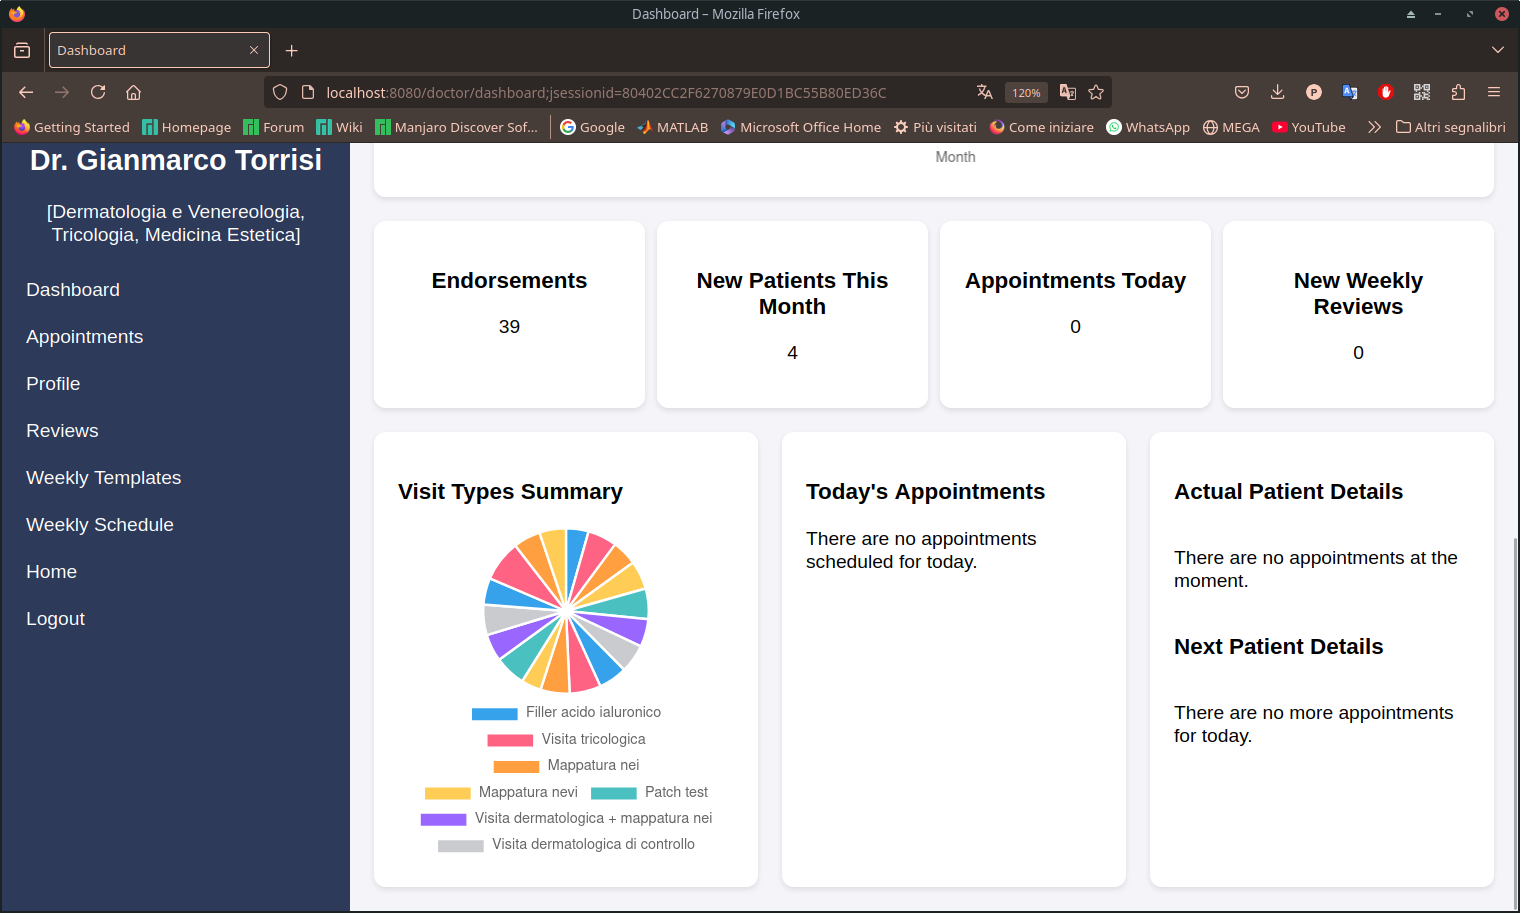
\includegraphics[scale=0.30]{resources/screenshots/doctor_ui/dashboard_bottom.png}
    \caption{Pie chart showing the distribution of services provided by the doctor.}
    \label{fig:services_piechart}
\end{figure}

The dashboard provides doctors with an overview of their current performance. It includes:
\begin{itemize}
    \item A line chart displaying total earnings for the current year.
    \item A pie chart illustrating the distribution of services provided.
    \item A summary of today's appointments, with access to detailed information.
    \item A preview of the next scheduled patient.
    \item Key performance indicators, including:
    \begin{itemize}
        \item \textbf{Endorsements}
        \item \textbf{New Patients This Month}
        \item \textbf{Appointments Today}
        \item \textbf{New Weekly Reviews}
    \end{itemize}
\end{itemize}

\subsection{Appointment List}
This section allows the doctor to view a comprehensive list of appointments. The list can be filtered by date, and each entry provides access to detailed information or cancellation options.

\begin{figure}[!h]
    \centering
    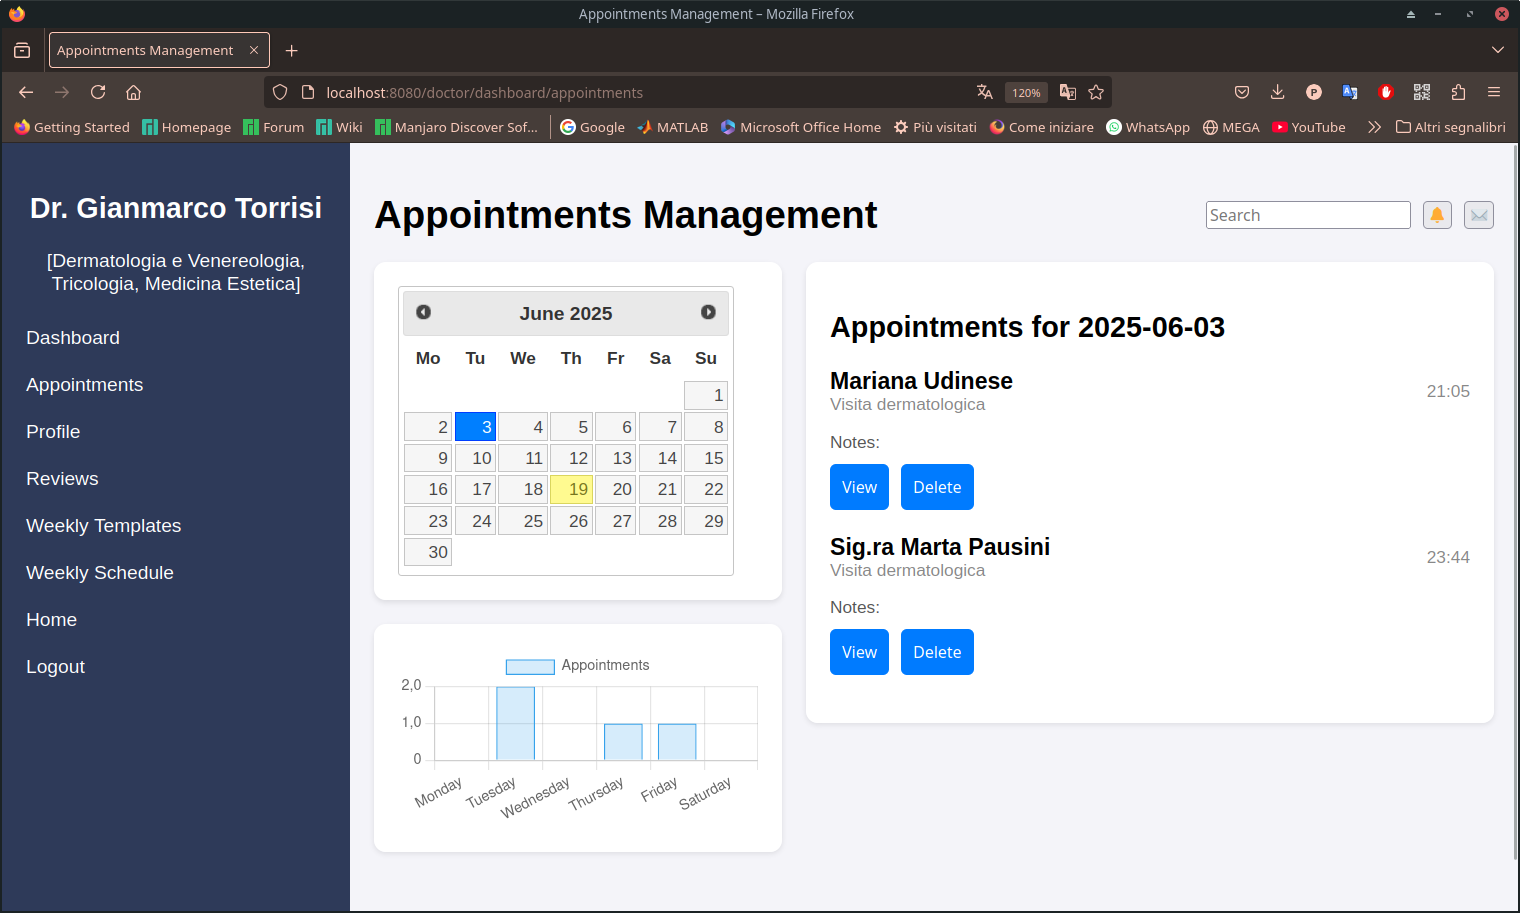
\includegraphics[scale=0.30]{resources/screenshots/doctor_ui/appointments.png}
    \caption{Appointment list with filtering options.}
    \label{fig:appointment_list}
\end{figure}

\subsection{Personal Profile}

\begin{figure}[!h]
    \centering
    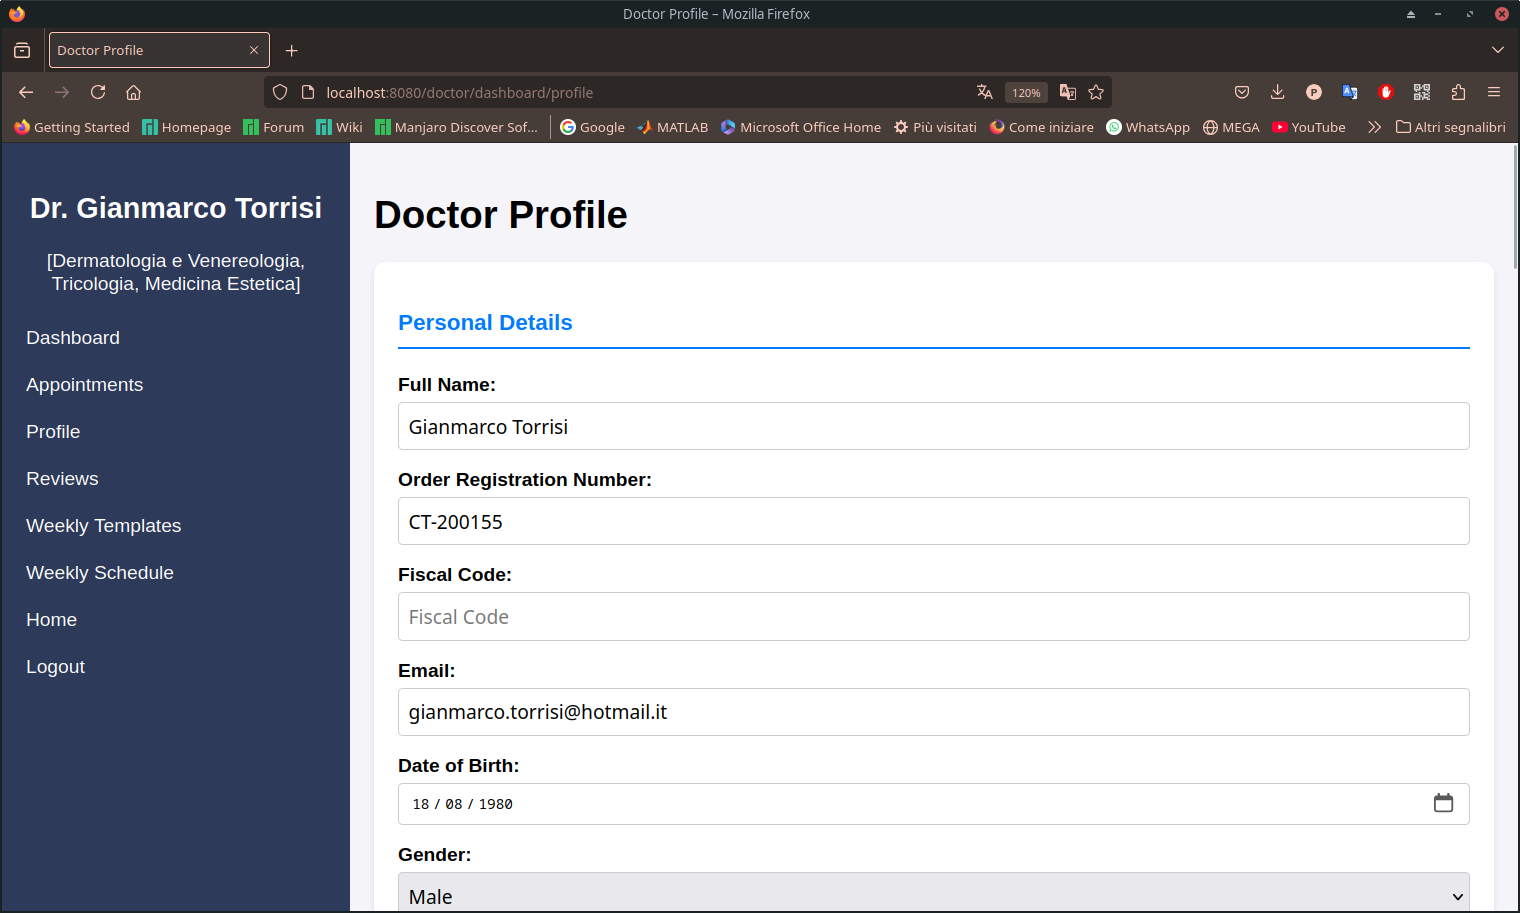
\includegraphics[scale=0.30]{resources/screenshots/doctor_ui/personal_info.png}
    \caption{Doctor's profile page with editable fields.}
    \label{fig:doctor_profile}
\end{figure}

\begin{figure}[!h]
    \centering
    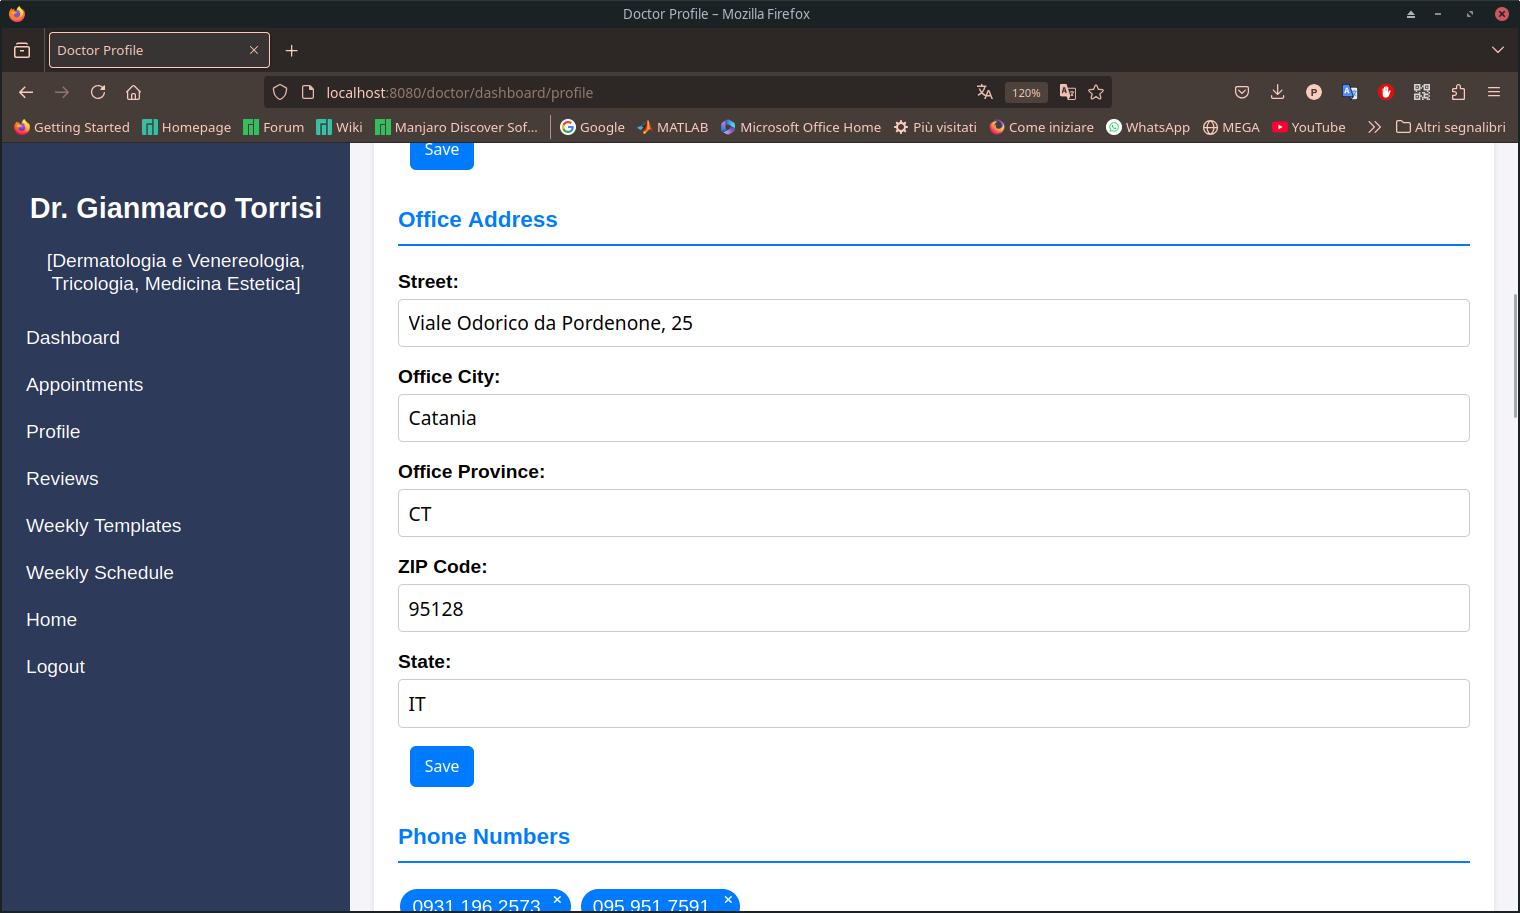
\includegraphics[scale=0.30]{resources/screenshots/doctor_ui/address.png}
    \caption{Doctor's office address and contact information.}
    \label{fig:doctor_address}
\end{figure}

\begin{figure}[!h]
    \centering
    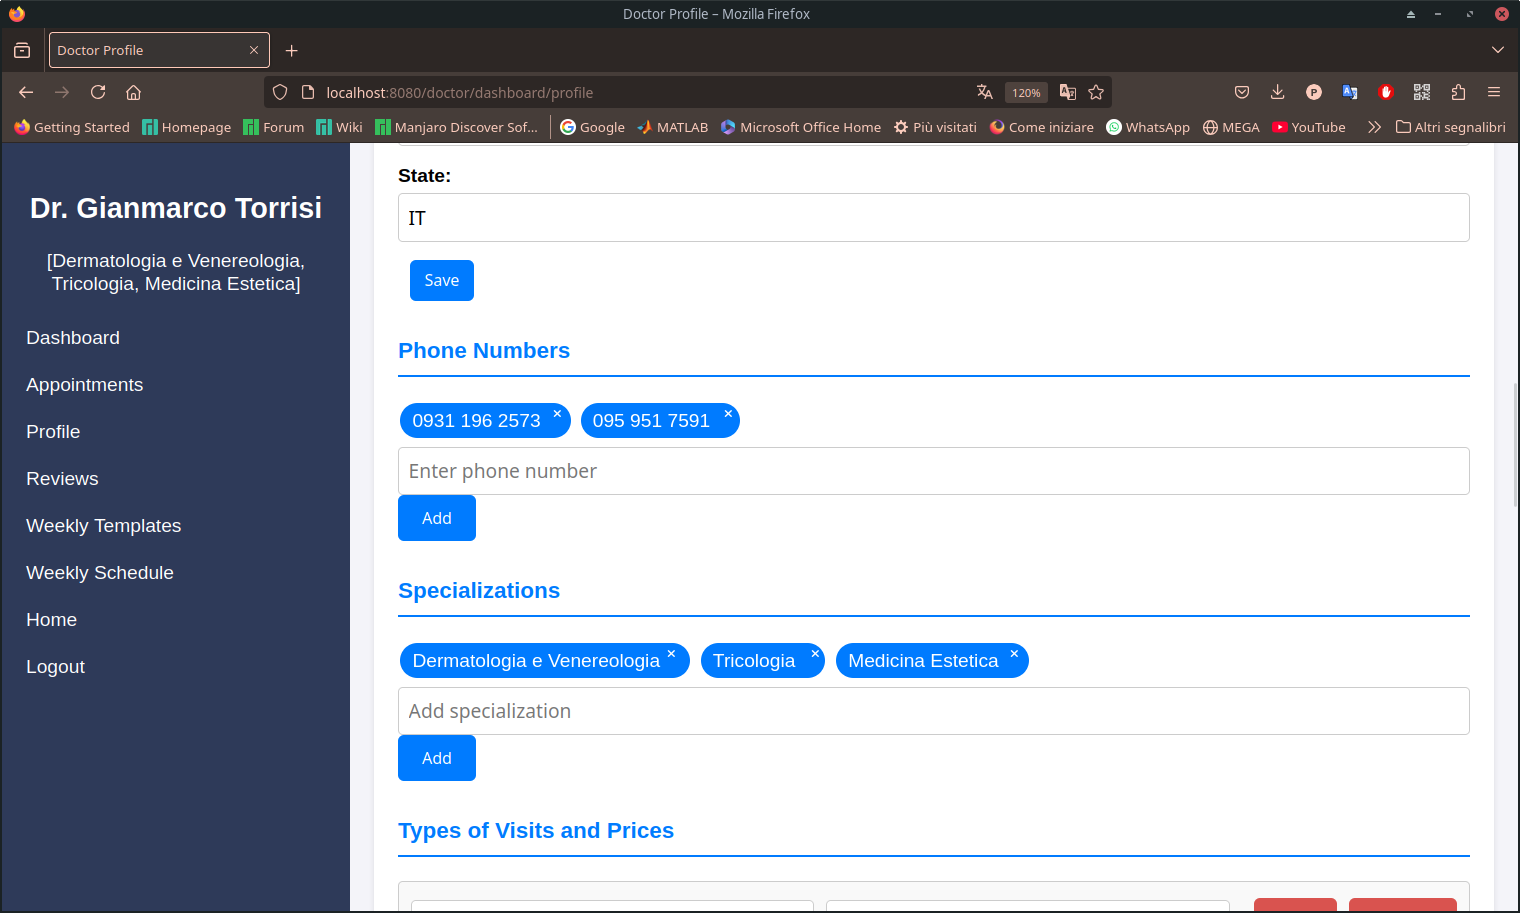
\includegraphics[scale=0.30]{resources/screenshots/doctor_ui/specializations.png}
    \caption{Medical specialties that the doctor can add or edit.}
    \label{fig:doctor_specialties}
\end{figure}

\begin{figure}[!h]
    \centering
    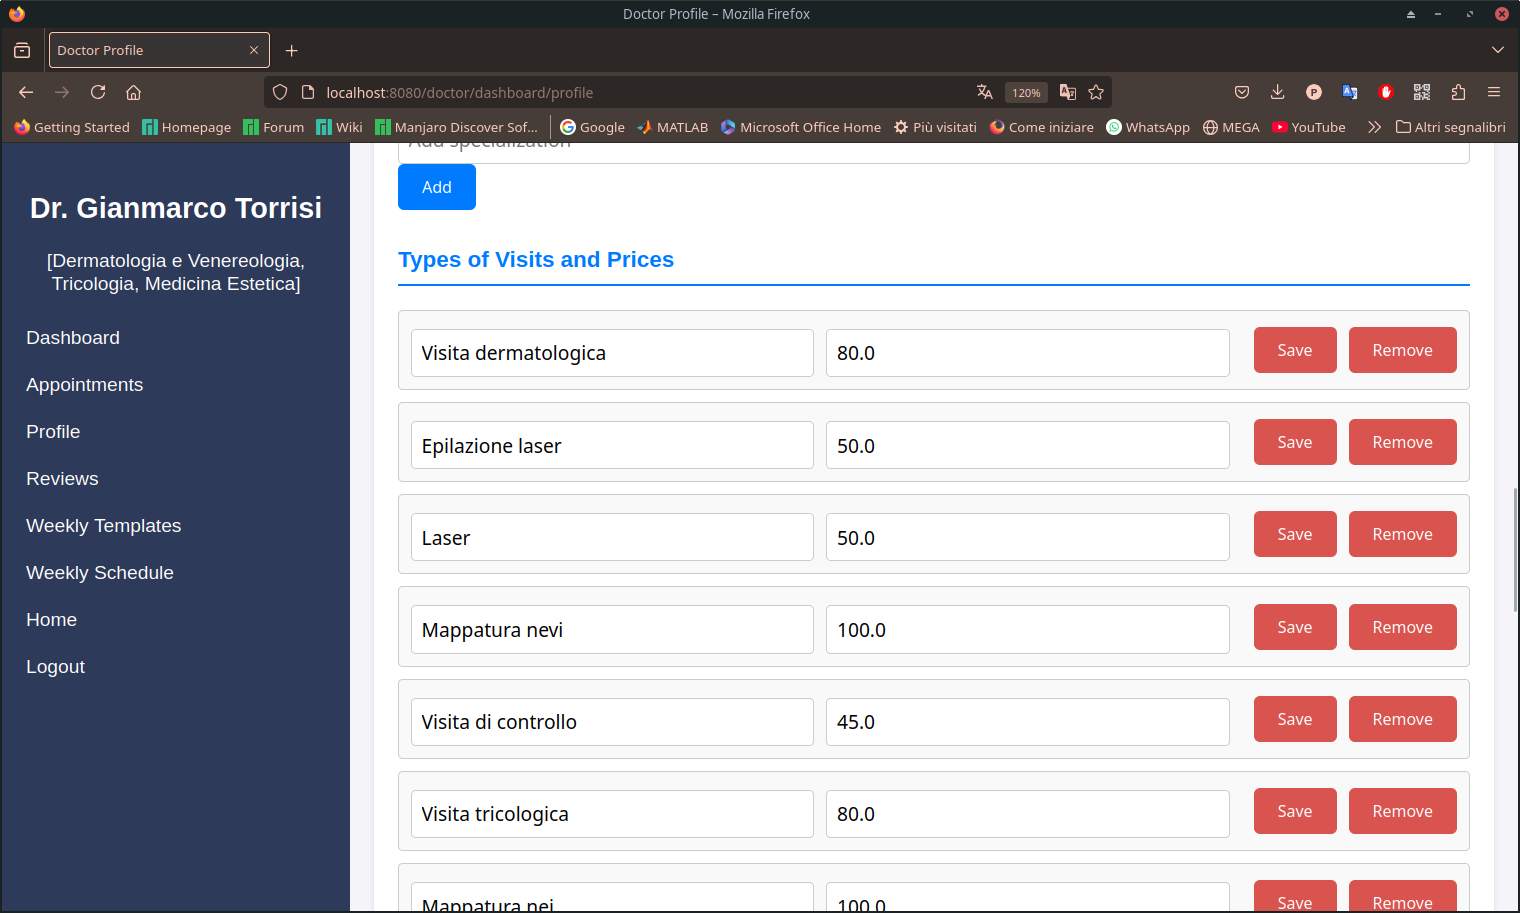
\includegraphics[scale=0.30]{resources/screenshots/doctor_ui/services.png}
    \caption{Services offered by the doctor, including name and cost.}
    \label{fig:doctor_services}
\end{figure}

In the profile section, doctors can view and edit their personal details and professional information. Specifically, they can:
\begin{itemize}
    \item Update their office address, phone numbers, and email address.
    \item Provide a list of services they offer, including the name and cost of each.
    \item Add or edit their medical specialties.
    \item Change their account password.
\end{itemize}

\subsection{Review Page}

\begin{figure}[!h]
    \centering
    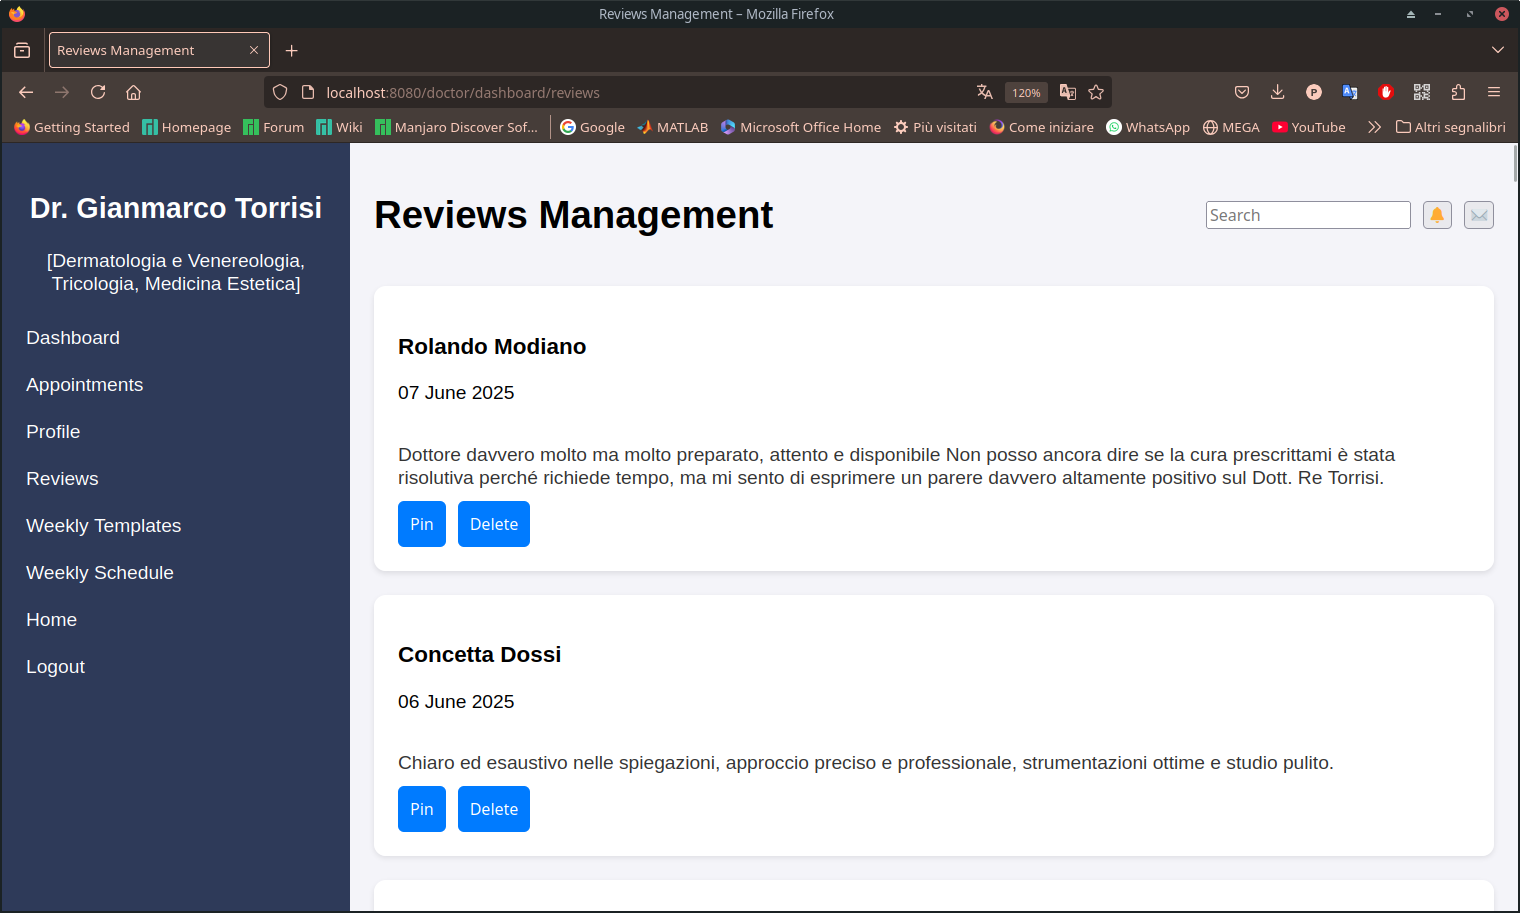
\includegraphics[scale=0.30]{resources/screenshots/doctor_ui/reviews.png}
    \caption{Patient reviews with options to delete or view details.}
    \label{fig:patient_reviews}
\end{figure}

Doctors can browse the reviews left by their patients. If necessary, inappropriate or outdated reviews can be deleted directly from this section.

\subsection{Calendar Templates}

\begin{figure}
    \centering
    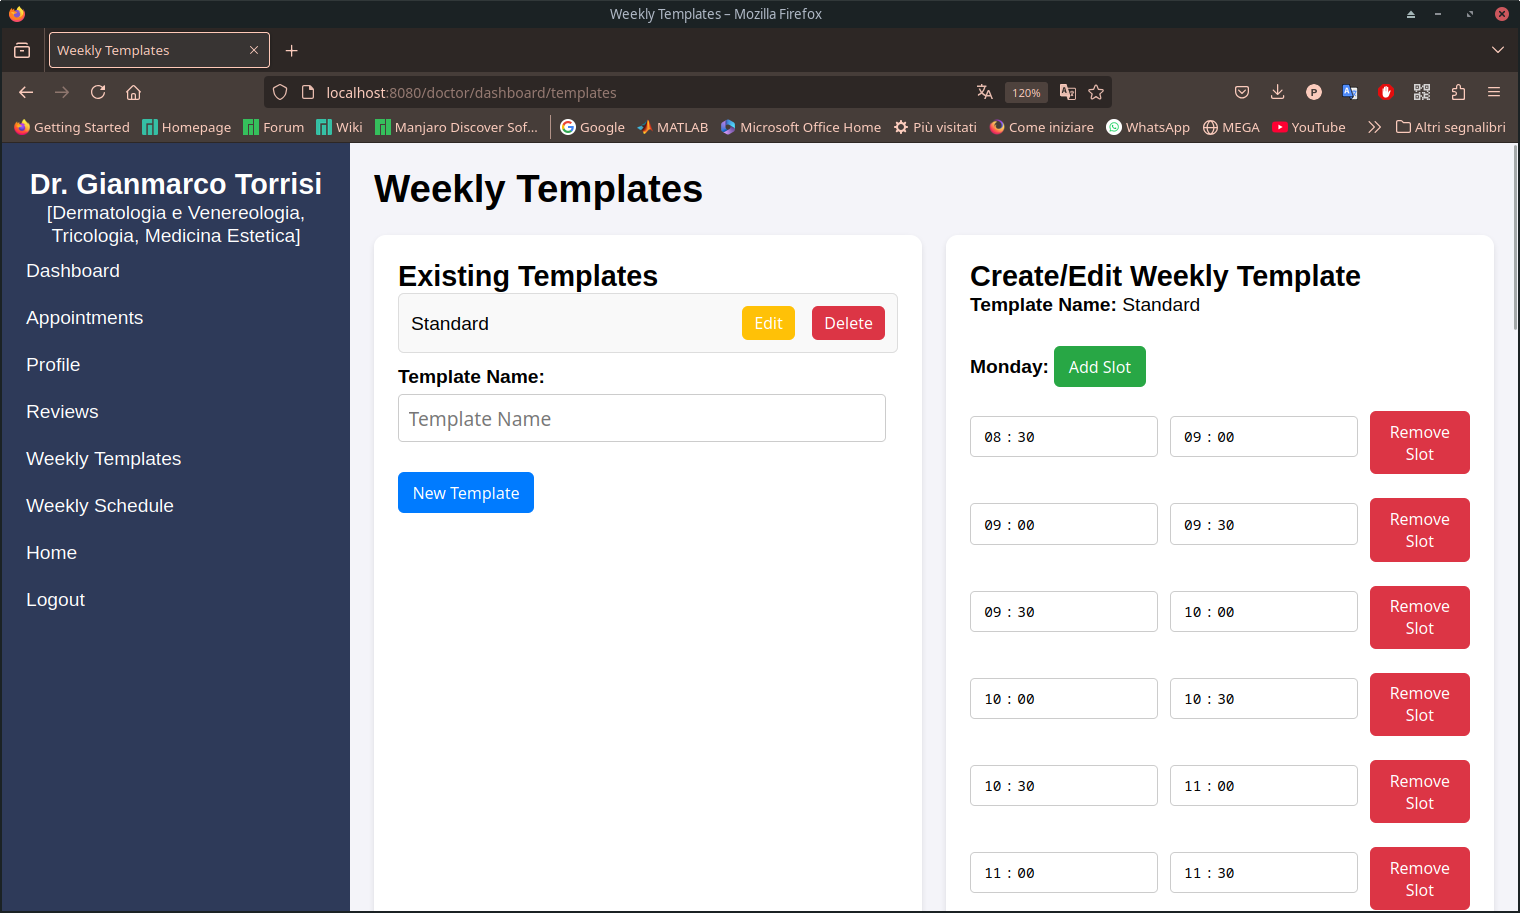
\includegraphics[scale=0.30]{resources/screenshots/doctor_ui/template.png}
    \caption{Calendar templates for managing weekly availability.}
    \label{fig:calendar_templates}
\end{figure}

In this area, doctors can create and manage calendar templates that define their weekly availability. Each template includes:
\begin{itemize}
    \item A custom name for the template.
    \item For each day of the week, a list of time slots indicating availability.
\end{itemize}
Templates can be edited or deleted at any time.

\subsection{Weekly Schedule}

\begin{figure}[!h]
    \centering
    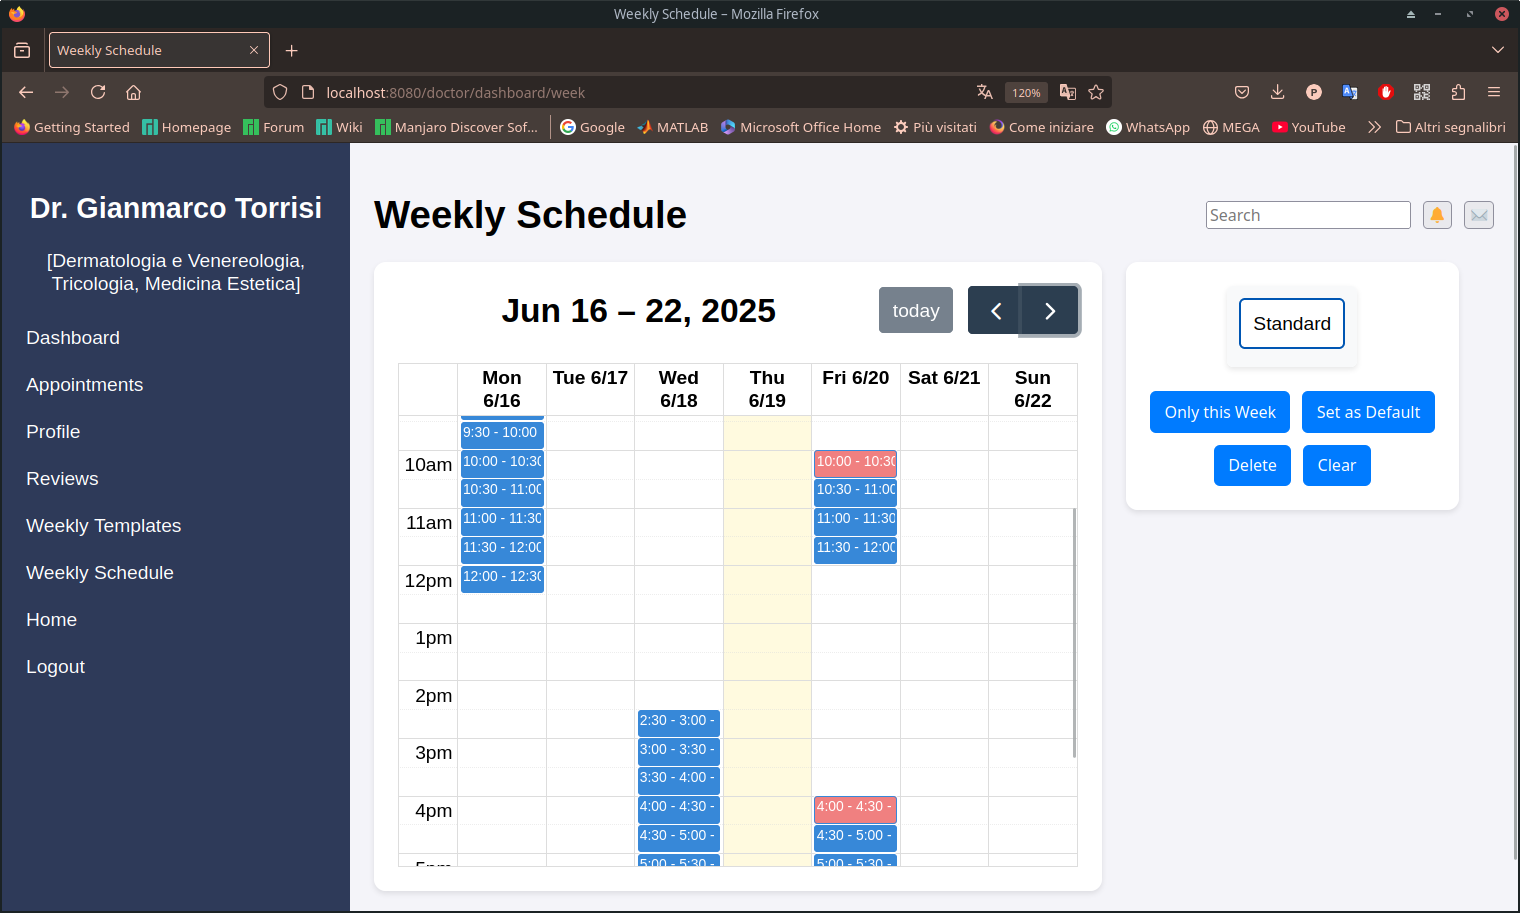
\includegraphics[scale=0.30]{resources/screenshots/doctor_ui/schedule.png}
    \caption{Weekly schedule with booked and available time slots.}
    \label{fig:weekly_schedule}
\end{figure}

The schedule page allows doctors to view and manage their weekly appointment calendar. Key features include:
\begin{itemize}
    \item Viewing existing appointments.
    \item Assigning a predefined calendar template to a specific week.
    \item Deleting the calendar for a selected week.
\end{itemize}

The calendar visually distinguishes between booked slots (highlighted in red) and available time slots (in blue), allowing for quick assessment and management.
